\subsection{Aprendizaje profundo}

El aprendizaje profundo se basa en el uso de grandes cantidades de datos, algoritmos de optimización, funciones de activación y arquitecturas específicas para cada problema, como las redes neuronales convolucionales, las redes neuronales recurrentes y las redes generativas adversarias, por mencionar algunos \cite{geron2019hands}. Se inspira en el funcionamiento del cerebro humano y permite a las computadoras procesar datos de forma no lineal, iterativa y jerárquica, extrayendo así niveles de abstracción y representación cada vez más altos y significativos \cite{goodfellow2016deep}.

En la actualidad, es aplicado a diversos dominios como la visión por computador, el reconocimiento de voz, la traducción automática, la robótica, la biología y la medicina, y ofrece ventajas en el descubrimiento de exoplanetas, nuevos fármacos y enfermedades, estudio de la genética humana, entre otros \cite{patterson2017deep}.

Varios autores como \citeA{elgendy2020deep}, ubican al aprendizaje profundo como un subconjunto de aprendizaje automático, tal y como lo muestra la Figura \ref{fig:ia}, esto debido a que utiliza técnicas de aprendizaje supervisado, no supervisado o por refuerzo para entrenar modelos complejos y de gran capacidad.

\begin{figure}[H]
    \begin{center}
        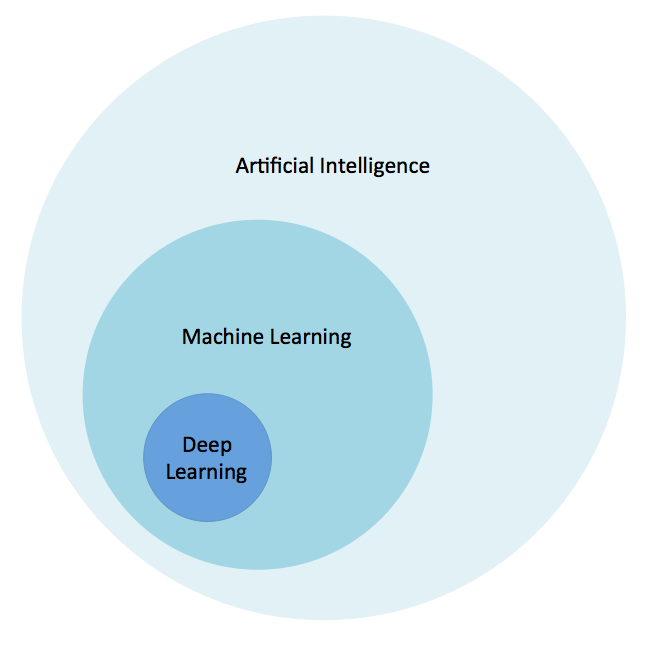
\includegraphics[width=0.6\textwidth]{Images/relation.png}
    \end{center}
    \caption{Diferencias entre inteligencia artificial (AI), aprendizaje automático (ML) y aprendizaje profundo (DL).}
    \reference{Datos tomados de \citeA{patterson2017deep}.}
    \label{fig:ia}
\end{figure}

Según \cite{patterson2017deep}, para que un algoritmo sea considerado como aprendizaje profundo debe cumplir con ciertas condiciones:

\begin{itemize} \item Mayor número de neuronas presentes que en redes anteriores. \item Formas más complejas de inter conectar neuronas y/o capas en la red. \item Extracción automática de características. \item Uso de una gran cantidad de recursos computacionales. \end{itemize}

El aprendizaje profundo se distingue por no requerir la intervención humana para extraer las características relevantes de los datos, sino que las aprende de forma automática mediante arquitecturas complejas. Estas características se usan luego para realizar tareas como clasificación, detección o generación, según se ilustra en la Figura~\ref{fig:comparasion}.

\begin{figure}[H]
    \begin{center}
        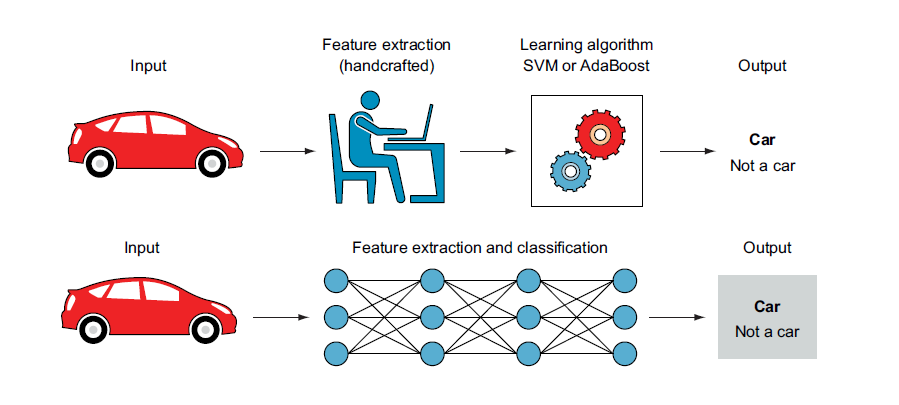
\includegraphics[width=1\textwidth]{Images/comparasion.png}
    \end{center}
    \caption{Diferencias entre el aprendizaje automático y el aprendizaje profundo.}
    \reference{Datos tomados de \citeA{elgendy2020deep}.}
    \label{fig:comparasion}
\end{figure}

Las redes neuronales son la base de los algoritmos de aprendizaje profundo. Estas redes se caracterizan por tener muchas capas que les permiten aumentar su profundidad y su capacidad de aprendizaje (de ahí el nombre ``profundo’'). Sin embargo, a mayor profundidad, mayor es el número de parámetros que se deben entrenar, lo que implica un mayor costo computacional y una mayor complejidad \cite{elgendy2020deep}.

\subsubsection{Redes neuronales artificiales (ANNs)}

Artificial Neural Networks en inglés, son algoritmos de inteligencia artificial inspirados en el funcionamiento de las neuronas biológicas, como se muestra en la Figura~\ref{fig:ComparacionNeurona} \cite{elgendy2020deep}.

\begin{figure}[H]
    \begin{center}
        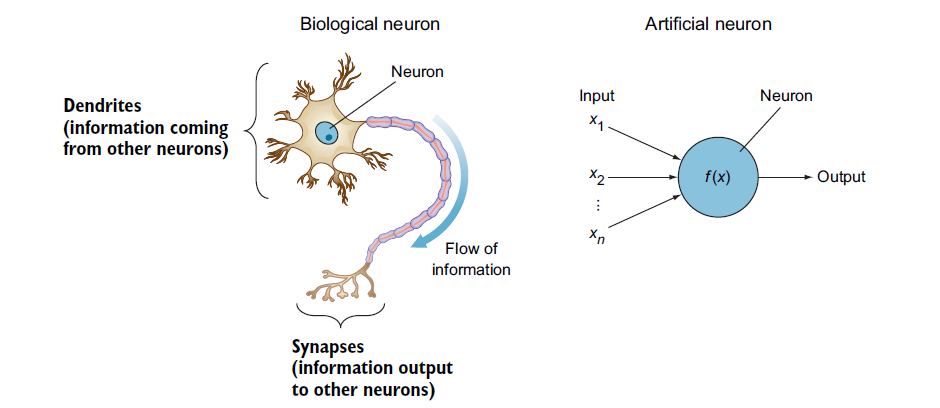
\includegraphics[width=1\textwidth]{Images/neuron.png}
    \end{center}
    \caption{Diferencias entre una neurona biológica y una neurona artificial.}
    \reference{Datos tomados de \citeA{elgendy2020deep}.}
    \label{fig:ComparacionNeurona}
\end{figure}

El perceptrón es el modelo más simple de red neuronal artificial, propuesto por Frank Rosenblatt en 1957. Se basa en una unidad de umbral lineal (LTU), que es una neurona artificial que calcula una combinación lineal de las entradas y las pesos sinápticos, y luego aplica una función de activación para obtener la salida. El perceptrón tiene una sola capa de neuronas, cada una conectada a todas las entradas del vector de características (ver Figura~\ref{fig:ann}).

\begin{figure}[H]
    \begin{center}
        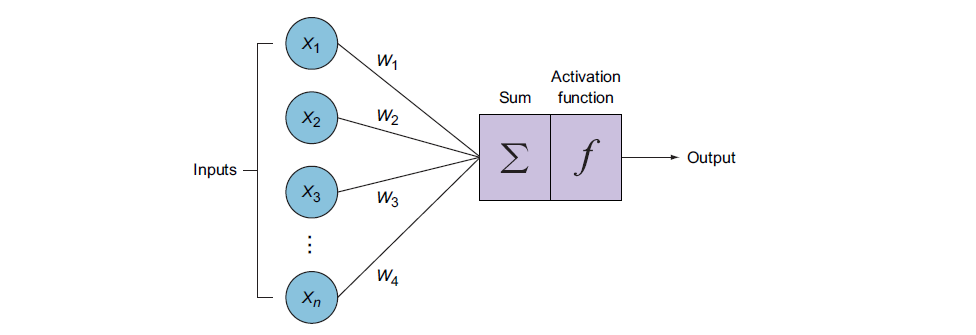
\includegraphics[width=1\textwidth]{Images/ann.png}
    \end{center}
    \caption{Arquitectura básica de una red neuronal artificial de una sola capa.}
    \reference{Datos tomados de \citeA{elgendy2020deep}.}
    \label{fig:ann}
\end{figure}

Para representar gráficamente estas conexiones, se usan neuronas especiales llamadas neuronas de entrada, que transmiten el valor que reciben. Además, se suele añadir un sesgo a cada neurona, que se modela mediante una neurona especial que siempre emite 1. El sesgo permite desplazar el umbral de activación de la neurona y mejorar su capacidad de adaptación \cite{geron2019hands}.

Cada neurona artificial recibe varias entradas y las pondera mediante unos pesos sinápticos, que son los parámetros que se ajustan mediante un algoritmo de aprendizaje basado en los resultados obtenidos. El objetivo del aprendizaje es que la red neuronal pueda aproximar una función que relacione las entradas con las salidas deseadas. Para ello, cada neurona artificial calcula una combinación lineal de las entradas y los pesos, y luego aplica una función de activación no lineal para obtener la salida \cite{patterson2017deep}. La ecuación que representa el cálculo de la salida de una neurona artificial es la siguiente:

\begin{equation} Z = f(W^T X + b) \end{equation}

Donde $Z$ es la salida de la neurona, $f$ es la función de activación, $W$ es el vector de pesos sinápticos, $X$ es el vector de entradas y $b$ es el sesgo.

\textbf{a) Perceptrón multicapa}

Es una arquitectura de red neuronal artificial que está compuesta por múltiples capas de neuronas. Cada capa puede tener más de una neurona, y estas pueden estar conectadas entre sí a través de pesos sinápticos. La arquitectura de este tipo de redes neuronales está compuesta por una capa de entrada, capas ocultas y una capa de salida \cite{geron2019hands}.

\begin{figure}[H]
    \begin{center}
        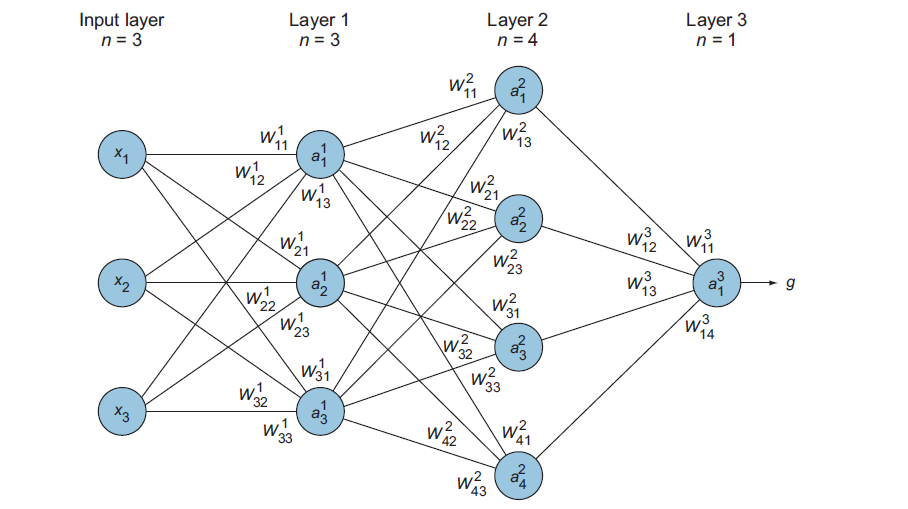
\includegraphics[width=1\textwidth]{Images/mlp.png}
    \end{center}
    \caption{Arquitectura de un perceptrón multicapa de 3 capas (1 capa de entrada, 2 capas ocultas + 1 capa de salida).}
    \reference{Datos tomados de \citeA{elgendy2020deep}.}
    \label{fig:mlp}
\end{figure}

La Figura~\ref{fig:mlp} ilustra una red neuronal artificial con entradas $X$, pesos $W$, neuronas $a$ y una salida $g$.

El proceso para obtener este último valor se llama propagación hacia adelante, y consiste en calcular la salida de cada capa de la red a partir de las entradas y los pesos, comparando la salida obtenida con la salida esperada, que se proporciona en un conjunto de datos.

Para medir la diferencia entre ambas salidas, se usa una función de error, que se busca minimizar mediante un algoritmo de optimización. Este algoritmo actualiza los pesos de la red, usando una técnica llamada propagación hacia atrás, que consiste en ajustar los pesos en sentido inverso, desde la capa de salida hasta la capa de entrada. Este ciclo se realiza hasta que la red alcance un nivel de precisión satisfactorio \cite{rashid2016make}.

\textbf{b) Funciones de activación}

Las funciones de activación buscan lograr la no linealidad de la red neuronal \cite{patterson2017deep}. Se utilizan para propagar la salida de los nodos de la capa anterior hacia la siguiente capa. Están inspiradas en el comportamiento de las neuronas biológicas, las cuales al lograr pasar un umbral emiten pulsaciones eléctricas a las demás neuronas conectadas, tratando a las neuronas que no alcancen el umbral como muertas, esto con el fin de proporcionar sólo la información relevante a la siguiente capa \cite{rashid2016make}.

Es deseable que una función de activación aproxime su función de identidad cerca al origen. La función de activación de una neurona está dada por:

\begin{equation}
    f(W^T X + b)
\end{equation}

Donde, $f$ es la función de activación, $W$ es el vector de pesos sinápticos, $X$ es el vector de entradas y $b$ es el sesgo. Usualmente, $W$ y $b$ son inicializados con valores cercanos a $0$ por el método de gradiente descendiente, por lo que $W^T X + b$ estará cerca a 0. Si $f$ aproxima su función de identidad a 0, su gradiente será aproximadamente igual a su entrada, haciendo que el algoritmo de entrenamiento converja más rápido \cite{aghdam2017guide}.

Dependiendo del tipo de gráfico que forme la función, se pueden clasificar en funciones sigmoideas (en forma de $S$), rectilíneas, por mencionar algunos.

\textbf{\textit{Sigmoidea:}} Esta determinada por la siguiente ecuación:

\begin{equation}
    f_{sigmoid}(x) = \frac{1}{1+e^{-x}}
\end{equation}

Su derivada está dada por:

\begin{equation}
    f^{'}_{sigmoid}(x) = f(x)(1-f(x))
\end{equation}

Donde, $ f_{sigmoid}(x): \mathbb{R} \rightarrow  [0,1] $.

La función sigmoidea es una función inspirada por comportamientos biológicos, por lo que fue muy usada en el diseño de redes neuronales \cite{aghdam2017guide}.

\begin{figure}[H]
    \begin{center}
        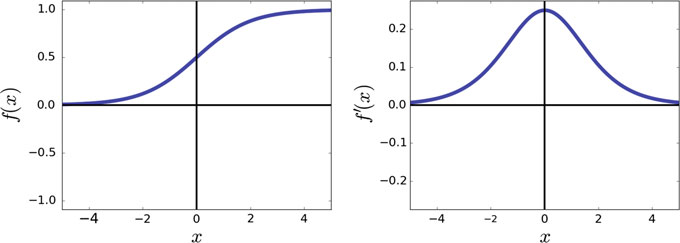
\includegraphics[width=0.7\textwidth]{Images/sigmoid.png}
    \end{center}
    \caption{Función de activación sigmoidea y su derivada correspondiente.}
    \reference{Datos tomados de \citeA{aghdam2017guide}.}
    \label{fig:sigmoid}
\end{figure}

En la Figura~\ref{fig:sigmoid} se muestra el gráfico de la función sigmoidea y su derivada.

\textbf{\textit{Tangente hiperbólica:}} Es una función re escalada de la función sigmoidea ya que su rango va desde -1 a 1 a diferencia de éste último. Esta determinada por la siguiente ecuación \cite{castaneda2019evaluation}:

\begin{equation}
    f_{tanh}(x) = \frac{e^{x}-e^{-x}}{e^{x}+e^{-x}} = \frac{1 - e^{-2x}}{1 + e^{-2x}}
\end{equation}

Su derivada está dada por:

\begin{equation}
    f^{'}_{tanh}(x) = 1 - f_{tanh}(x)^{2}
\end{equation}

Donde, $  f_{sigmoid}(x) : \mathbb{R} \rightarrow  [-1,1] $.

Además, a diferencia de la función sigmoidea, la función tangente hiperbólica aproxima su función de identidad al origen, tal y como se muestra en la Figura~\ref{fig:tangent}, esta propiedad hace posible incrementar la convergencia del algoritmo de gradiente descendiente \cite{aghdam2017guide}.

\begin{figure}[H]
    \begin{center}
        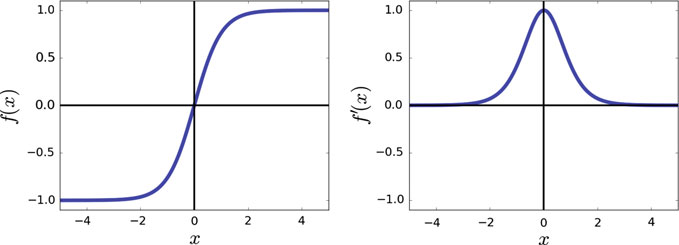
\includegraphics[width=0.7\textwidth]{Images/tangent.png}
    \end{center}
    \caption{Función de activación tangente hiperbólica y su derivada correspondiente.}
    \reference{Datos tomados de \citeA{aghdam2017guide}.}
    \label{fig:tangent}
\end{figure}

Sin embargo, esta función es propensa a caer en problemas de desvanecimiento de gradiente si la red neuronal presenta muchas capas, ya que al incrementarse el valor de $x$ la función devuelve valores saturados  \cite{aghdam2017guide}.

\textbf{\textit{Softsign:}} Esta función de activación es similar a la función tangente hiperbólica, ya que su rango también va de -1 a 1. La ecuación que representa la función es la siguiente:

\begin{equation}
    f_{softsign}(x) = \frac{x}{1 + |x|}
\end{equation}

Su derivada está dada por:

\begin{equation}
    f^{'}_{softsign}(x) = \frac{1}{(1 + |x|)^{2}}
\end{equation}

\begin{figure}[H]
    \begin{center}
        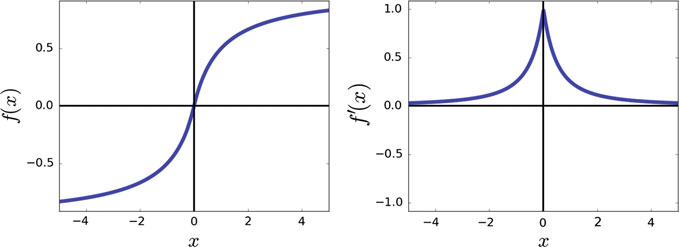
\includegraphics[width=0.7\textwidth]{Images/softsign.png}
    \end{center}
    \caption{Función de activación softsign y su derivada correspondiente.}
    \reference{Datos tomados de \citeA{aghdam2017guide}.}
    \label{fig:softsign}
\end{figure}

Como se puede observar en la Figura~\ref{fig:softsign}, la función de identidad se aproxima al origen y su derivada en este punto toma el valor de 1. Sin embargo, presenta el mismo problema de desvanecimiento de gradiente si la red neuronal presenta muchas capas, aunque en menor medida que la función de tangente hiperbólica. Además, computacionalmente requiere de menos recursos que éste último \cite{aghdam2017guide}.

\textbf{\textit{Softmax:}} Se utiliza habitualmente en la capa de salida de los clasificadores para obtener una distribución de probabilidad sobre diferentes clases. Para un vector \( \mathbf{x} \) en un espacio de \( K \) dimensiones, la función softmax se define como:

\begin{equation}
    f_{softmax}(\mathbf{x})_i = \frac{e^{x_i}}{\sum_{k=1}^{K} e^{x_k}}
\end{equation}

donde \( i = 1, \ldots, K \) y \( x_i \) representa el elemento i-ésimo del vector \( \mathbf{x} \).

La derivada de la función softmax con respecto a cada elemento \( x_i \) depende de todos los componentes del vector \( \mathbf{x} \), reflejado en la siguiente forma para la derivada parcial de \( f_{softmax}(\mathbf{x})_i \) con respecto a \( x_j \):

\begin{equation}
    \frac{\partial f_{softmax}(\mathbf{x})_i}{\partial x_j} =
    \begin{cases}
        f_{softmax}(\mathbf{x})_i \cdot (1 - f_{softmax}(\mathbf{x})_i) & \text{si } i = j,    \\
        -f_{softmax}(\mathbf{x})_i \cdot f_{softmax}(\mathbf{x})_j      & \text{si } i \neq j.
    \end{cases}
\end{equation}

Esta función es especialmente útil en problemas de clasificación multi clase y es menos propensa al problema del desvanecimiento de gradiente, especialmente cuando se utiliza en conjunto con la función de pérdida de entropía cruzada \cite{goodfellow2016deep}.

\textbf{\textit{ReLU:}} Es generalmente utilizada en redes neuronales profundas. Las funciones de activación mencionadas anteriormente tienen a desvanecer en la etapa de retro propagación cuando la red presenta muchas capas \cite{aghdam2017guide}. Una ReLU está dada por:

\begin{equation}
    f_{relu}(x) = max(0,x)
\end{equation}

Su derivada está dada por:

\begin{equation}
    {f}'_{relu}(x) = \left\{\begin{matrix}
        0 & x < 0         \\
        1 & x \geqslant 0
    \end{matrix}\right.
\end{equation}

\begin{figure}[H]
    \begin{center}
        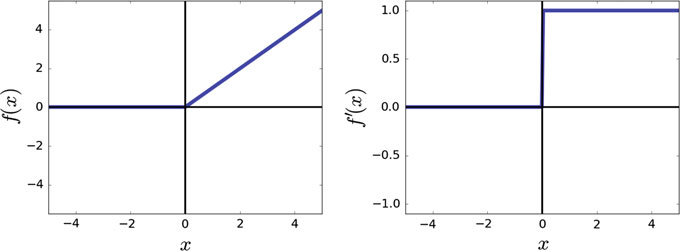
\includegraphics[width=0.7\textwidth]{Images/relu.png}
    \end{center}
    \caption{Función de activación ReLU y su derivada correspondiente.}
    \reference{Datos tomados de \citeA{aghdam2017guide}.}
    \label{fig:relu}
\end{figure}

Esta función no lineal funciona muy bien en la práctica, su derivada cuando $ \mathbb{R}^{+}$ siempre es 1 y no se satura cuando $ \mathbb{R}^{+}$ por lo que no presenta el problema de desvanecimiento de gradiente. Esto significa que el rango de esta función de activación es $[0, \infty)$. Al no tener este problema, se considera una buena opción para entrenar redes profundas. En el caso de las neuronas muertas, esta función siempre retorna un 0 haciéndola computacionalmente más eficiente. Sin embargo, esto puede afectar el nivel de exactitud general de la red \cite{aghdam2017guide}.

\textbf{\textit{Leaky ReLU:}} Busca resolver el problema de las neuronas muestras presentes en la función ReLU. La función leaky ReLU está dada por:

\begin{equation}
    {f}_{rrelu}(x) = \left\{\begin{matrix}
        \alpha x & x < 0         \\
        x        & x \geqslant 0
    \end{matrix}\right.
\end{equation}

Y su derivada por:

\begin{equation}
    {f}'_{rrelu}(x) = \left\{\begin{matrix}
        \alpha & x < 0         \\
        1      & x \geqslant 0
    \end{matrix}\right.
\end{equation}

\begin{figure}[H]
    \begin{center}
        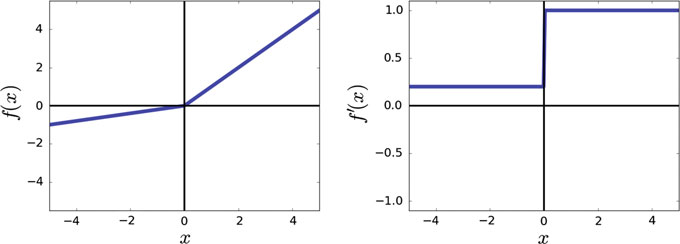
\includegraphics[width=0.7\textwidth]{Images/leaky-relu.png}
    \end{center}
    \caption{Función de activación Leaky ReLU y su derivada correspondiente.}
    \reference{Datos tomados de \citeA{aghdam2017guide}.}
    \label{fig:leaky-relu}
\end{figure}

Leaky ReLU asigna una pendiente a su entrada negativa (ver Figura~\ref{fig:leaky-relu}), la cual, puede tomar un valor entre [0,1] \cite{castaneda2019evaluation}. Generalmente, éste valor se establece en $ \alpha = 0.01 $. Sin embargo, según \cite{xu2015empirical}, se tiene mejor desempeño si se le asignan valores más altos al trabajar con algunos conjuntos de datos. En la práctica la función ReLU y leaky ReLU producen resultados similares, esto se debe a que las regiones positivas de ambas funciones son idénticas \cite{aghdam2017guide}.

\textbf{c) Funciones de pérdida}

Las redes neuronales utilizan funciones de pérdida para evaluar la discrepancia entre las predicciones y los valores reales. Dos de las funciones de pérdida más comunes son el Error Cuadrático Medio (MSE) y la Entropía Cruzada.

\textbf{\textit{Error Cuadrático Medio (MSE)}}: El MSE mide la diferencia cuadrática promedio entre las predicciones \(\hat{y}_i\) y las etiquetas reales \(y_i\). Su fórmula es:

\begin{equation}
    MSE(W, b) = \frac{1}{n} \sum_{i=1}^{n} (y_i - \hat{y}_i)^2
\end{equation}

Donde \(n\) es el número de ejemplos. El MSE es sensible a valores atípicos, por lo que a veces se prefiere el Error Absoluto Medio (MAE), que calcula el promedio de los valores absolutos de los errores.

\textbf{\textit{Entropía Cruzada}}: Esta función mide la diferencia entre dos distribuciones probabilísticas, como la distribución real y la predicha por la red. Su fórmula es:

\begin{equation}
    CrossEntropy(W, b) = -\frac{1}{n} \sum_{i=1}^{n} \sum_{j=1}^{m} y_{ij} \log(\hat{y}_{ij})
\end{equation}

Aquí, \(m\) es el número de clases, y \(y_{ij}\) y \(\hat{y}_{ij}\) representan la realidad y la probabilidad predicha, respectivamente.

\textbf{d) Optimización}

Para optimizar una red neuronal, se busca minimizar su función de pérdida.

\textbf{\textit{Descenso del Gradiente}}: Este método actualiza los parámetros de la red (pesos \(W\) y sesgos \(b\)) de manera iterativa para minimizar la función de pérdida.

\begin{figure}[H]
    \begin{center}
        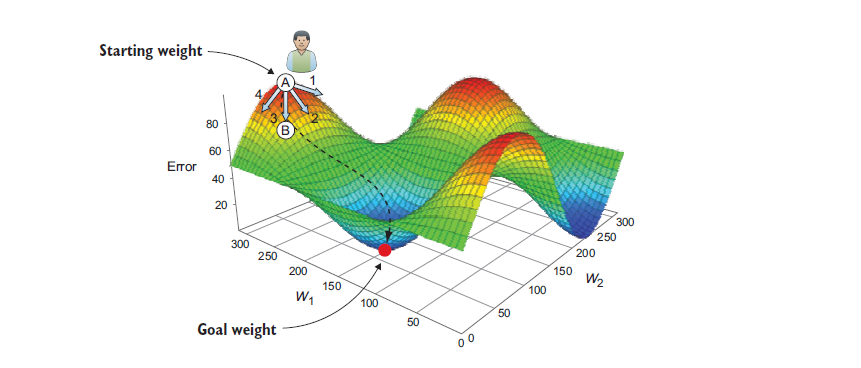
\includegraphics[width=\textwidth]{Images/Gradiente.png}
    \end{center}
    \caption{Descenso de gradiente.}
    \label{fig:Gradiente}
    \reference{Datos tomados de \citeA{elgendy2020deep}.}
\end{figure}

Existen varias variantes del descenso de gradiente:

\begin{itemize}
    \item \textit{Descenso del Gradiente por Lotes}: Utiliza todo el conjunto de datos para cada actualización de parámetros. Es eficiente para conjuntos de datos pequeños, pero menos práctico para grandes volúmenes de datos.
    \item \textit{Descenso de Gradiente Estocástico (SGD)}: Actualiza los parámetros para cada ejemplo individual, lo que lo hace más adecuado para grandes conjuntos de datos y capaz de escapar de mínimos locales.
    \item \textit{Descenso de Gradiente Mini-Lote}: Combina los enfoques anteriores, actualizando los parámetros para un subconjunto del conjunto de datos, equilibrando eficiencia y convergencia.
\end{itemize}

La elección entre estas variantes depende del tamaño del conjunto de datos y de las características específicas del problema.

\textbf{e) Retro propagación}

La retro propagación es el proceso utilizado para calcular los gradientes necesarios para el descenso de gradiente \cite{rashid2016make}.

Durante la retro propagación, los gradientes de la función de pérdida con respecto a los pesos \(W\) y sesgos \(b\) se calculan mediante la regla de la cadena. Posteriormente, estos gradientes se utilizan para actualizar los pesos y sesgos, optimizando así el rendimiento de la red.

\textbf{\textit{Ecuaciones de retro propagación}}:

Para la última capa \(L\):

\begin{equation}
    \delta^{(L)} = \nabla_a Cost \odot \sigma'(z^{(L)})
\end{equation}

Para las capas anteriores \(l < L\):

\begin{equation}
    \delta^{(l)} = ((W^{(l+1)})^T \delta^{(l+1)}) \odot \sigma'(z^{(l)})
\end{equation}

Donde \(\delta^{(l)}\) es el vector de error para la capa \(l\), \(W^{(l+1)}\) son los pesos de la capa siguiente, \(z^{(l)}\) son las entradas a las neuronas en la capa \(l\), y \(\sigma'\) es la derivada de la función de activación.

Esta metodología asegura que cada paso del aprendizaje se enfoque en reducir la función de pérdida, guiando así a la red hacia una mejor precisión en la tarea que realiza.

\subsubsection{Redes Neuronales Convolucionales (CNNs)}
Son arquitecturas de redes neuronales diseñadas específicamente para procesar datos en formato de matriz bidimensional, como las imágenes. Estas estructuras de red se componen de varias capas que aplican filtros (convoluciones) a los datos de entrada para extraer características significativas \cite{geron2019hands}.

\begin{figure}[H]
    \begin{center}
        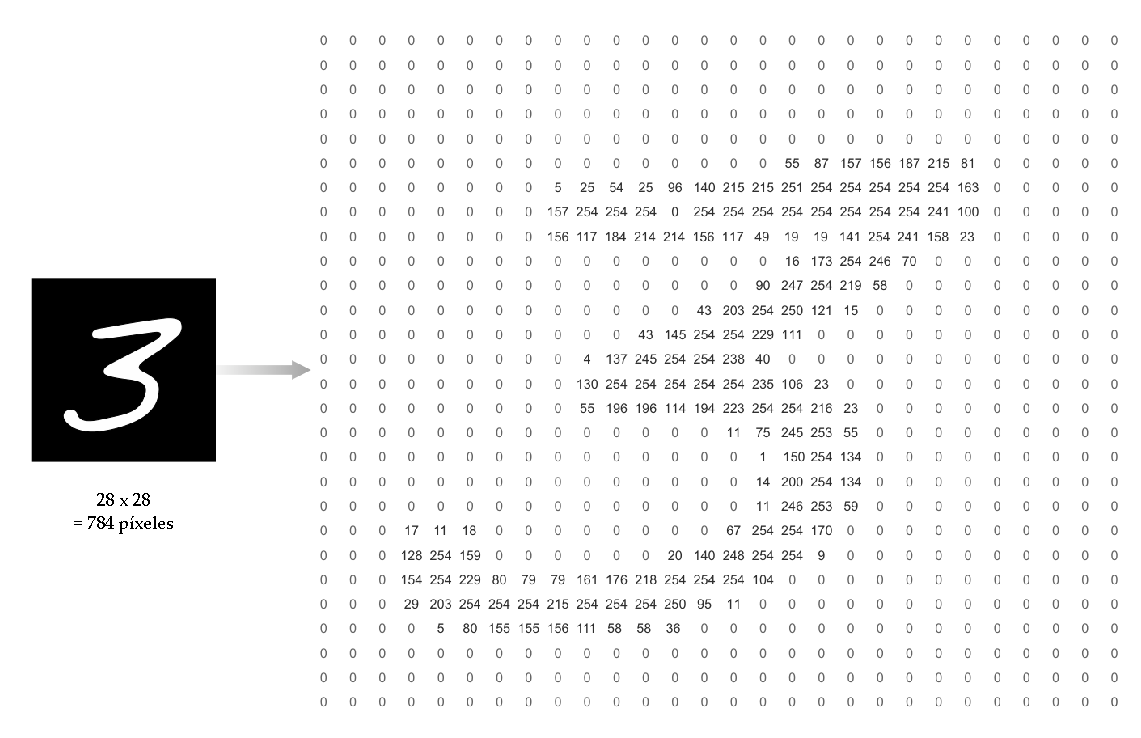
\includegraphics[width=\textwidth]{Images/ComposicionImagen.pdf}
    \end{center}
    \caption{Representación digital de una imagen.}
    \label{fig:ComposicionImagen}
    \reference{Datos tomados de \citeA{elgendy2020deep}.}
\end{figure}

Como se muestra en la Figura~\ref{fig:ComposicionImagen}, una imagen digital se representa mediante una matriz de píxeles, cada uno con un valor de intensidad asignado. Las imágenes de alta resolución presentan una entrada con alta dimensionalidad \cite{elgendy2020deep}. En redes neuronales tradicionales, cada píxel se conecta a muchas neuronas, con cada conexión representando un parámetro ajustable, resultando en un modelo con un número elevado de parámetros. Esto puede aumentar la carga computacional y propiciar el sobre ajuste \cite{rashid2016make}.

\begin{figure}[H]
    \begin{center}
        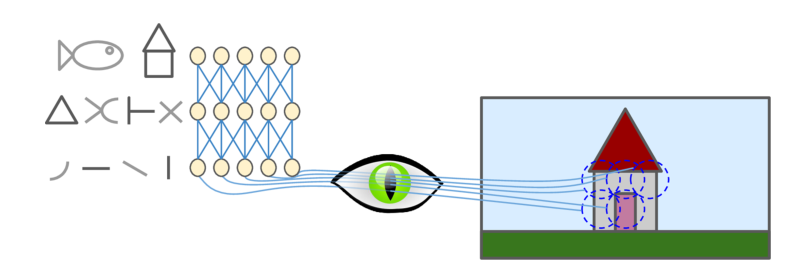
\includegraphics[width=\textwidth]{Images/VisionCNN.png}
    \end{center}
    \caption{Extracción de características de una imagen mediante el sistema visual humano.}
    \label{fig:VisionCNN}
    \reference{Datos tomados de \citeA{geron2019hands}.}
\end{figure}

Las CNNs manejan la alta dimensionalidad de las imágenes utilizando filtros convolucionales para procesar la matriz de píxeles, reduciendo así la dimensionalidad de los datos y extrayendo automáticamente características clave como bordes, texturas y colores. Este proceso es análogo a cómo el sistema visual humano interpreta información visual, ilustrado en la Figura~\ref{fig:VisionCNN}. Esto conduce a una reducción en el número de parámetros y la complejidad computacional, aumentando la eficiencia y evitando el sobre ajuste \cite{geron2019hands}.

La arquitectura fundamental de una CNN se muestra en la Figura~\ref{fig:ArquitecturaCNN}.

\begin{figure}[H]
    \begin{center}
        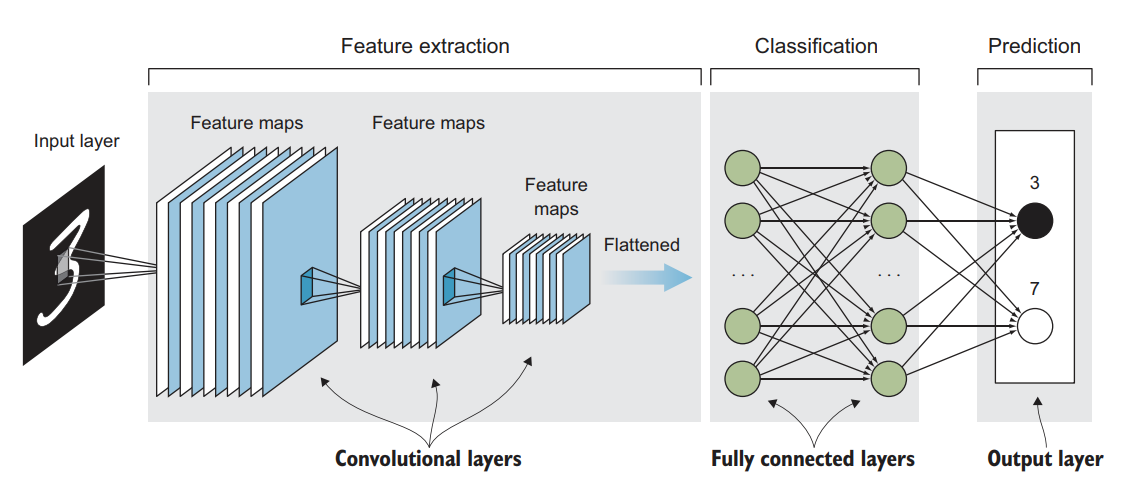
\includegraphics[width=\textwidth]{Images/ArquitecturaCNN.png}
    \end{center}
    \caption{Arquitectura base de una red neuronal convolucional.}
    \label{fig:ArquitecturaCNN}
    \reference{Datos tomados de \citeA{elgendy2020deep}.}
\end{figure}

Dentro de la arquitectura de una CNN, se encuentra el extractor de características, que incluye capas convolucionales y de agrupación (pooling). Las capas convolucionales identifican patrones locales en imágenes, como bordes o texturas, mientras que el agrupamiento reduce la dimensionalidad espacial, conservando las características más destacadas. La clasificación se realiza en las capas totalmente conectadas, que usan un vector de características aplanado para calcular las probabilidades de cada clase. Finalmente, la capa de salida produce predicciones probabilísticas de clases, ofreciendo una interpretación numérica de la probabilidad de que una imagen pertenezca a una clase específica \cite{elgendy2020deep}.

\textbf{a) Capas de entrada y salida}

La capa de entrada en una CNN consiste en las imágenes a procesar, representadas como matrices numéricas correspondientes a los valores de píxeles en canales de color, comúnmente rojo, verde y azul (RGB). Esta capa prepara las imágenes para su procesamiento en la red, estandarizando sus dimensiones para adecuarse a la arquitectura de la red \cite{rashid2016make, geron2019hands}.

La capa de salida en una CNN está orientada a proporcionar los resultados del proceso de clasificación. Para la clasificación de imágenes, esta capa suele emplear una función de activación softmax, generando un vector de probabilidades. Cada elemento de este vector indica la probabilidad de que la imagen corresponda a una de las clases predefinidas. La dimensión de esta capa es igual al número de clases que el modelo está capacitado para identificar \cite{geron2019hands}.

\textbf{b) Capas convolucionales}

Las capas convolucionales en una red neuronal convolucional utilizan filtros o kernels que se desplazan a través de la entrada para generar mapas de características, detectando patrones locales como texturas y bordes. La configuración de estos filtros influye en las características que se extraen \cite{rashid2016make, geron2019hands}.

\textbf{\textit{Convolución:}} Durante la convolución, un filtro se aplica sobre la imagen de entrada, desplazándose y realizando operaciones matemáticas para producir un valor en el mapa de características \cite{aghdam2017guide}.

\begin{figure}[H]
    \begin{center}
        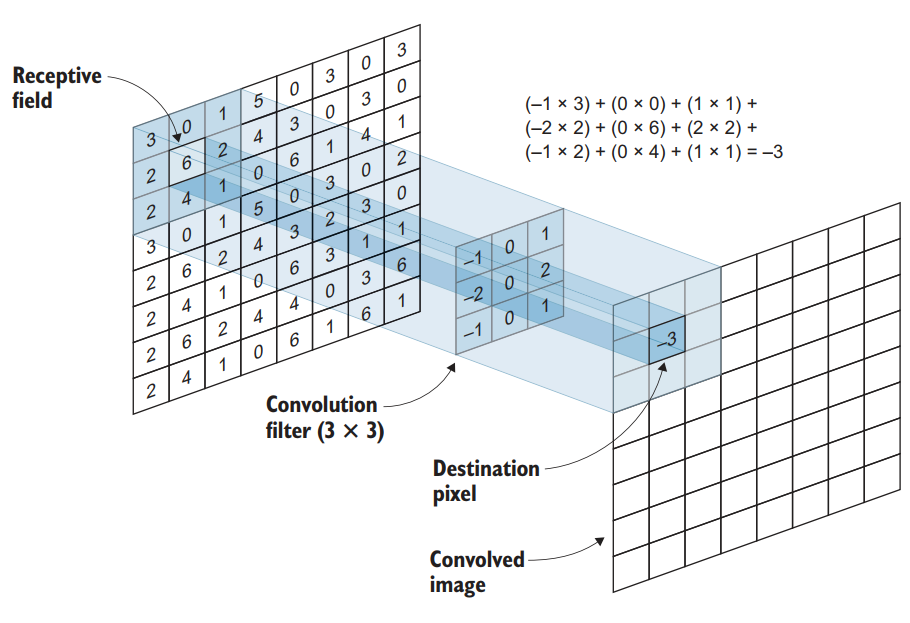
\includegraphics[width=\textwidth]{Images/CapaConvolucion.png}
    \end{center}
    \caption{Proceso de convolución en una red neuronal convolucional.}
    \label{fig:CapaConvolucion}
    \reference{Datos tomados de \citeA{elgendy2020deep}.}
\end{figure}

\textbf{\textit{Stride:}} El stride define el desplazamiento del filtro a lo largo de la entrada. Un stride mayor implica saltos más grandes del filtro, resultando en un mapa de características de menor tamaño. La fórmula para calcular el tamaño de salida sin considerar el padding es:

\begin{equation}
    \label{ecu:conv_stride_sin_padding}
    n_{salida} = \left[ \frac{n_{entrada} - n_{filtro}}{stride} + 1 \right]
\end{equation}

Donde \( n_{entrada} \) es el tamaño de la entrada y \( n_{filtro} \) el tamaño del filtro.

\textbf{\textit{Padding:}} El padding se utiliza para añadir bordes adicionales a la entrada, permitiendo que el filtro se aplique por completo incluso en los bordes, y manteniendo así el tamaño original de la imagen. Con padding, la fórmula para calcular el tamaño de salida se ajusta a:

\begin{equation}
    \label{ecu:conv_stride_con_padding}
    n_{salida} = \left[ \frac{n_{entrada} - n_{filtro} + 2 \times padding}{stride} + 1 \right]
\end{equation}

Donde \( padding \) representa el número de píxeles agregados alrededor de la entrada.

\textbf{\textit{Funciones de Activación Intermedias:}} Tras la convolución, las funciones de activación, como ReLU (Rectified Linear Unit), se aplican a los vectores de características para introducir no linealidades, permitiendo a la red aprender y representar datos más complejos. La función ReLU se define como:

\begin{equation}
    \label{ecu:relu}
    ReLU(x) = max(0, x)
\end{equation}

Donde \( x \) es el valor de entrada a la función de activación.

\textbf{c) Capas de agrupación (Pooling)}

Buscan reducir las dimensiones espaciales de las entradas sin alterar su profundidad. Esta técnica, al disminuir la cantidad total de datos, mejora la eficiencia computacional y reduce el número de parámetros del modelo, lo que ayuda a prevenir el sobre ajuste. Además, proporciona invariancia a traslaciones, mejorando la habilidad del modelo para reconocer patrones independientemente de su ubicación en la imagen \cite{geron2019hands, patterson2017deep}.

El proceso de agrupación emplea un kernel de pooling que se desplaza sobre la entrada con un stride específico. El tipo más común es el max pooling, que selecciona el valor máximo dentro del área cubierta por el kernel (ver Figura~\ref{fig:2-pooling}). Sin embargo, existen otros tipos de pooling, como el average pooling y el stochastic pooling, cada uno con sus propias características y aplicaciones \cite{scherer2010evaluation, zeiler2013stochastic}.

La ecuación para calcular el tamaño de salida de una capa de agrupación es la siguiente:

\begin{equation}
    \label{ecu:pooling_output}
    n_{salida} = \left[ \frac{n_{entrada} - n_{kernel} + 2 \times padding}{stride} + 1 \right]
\end{equation}

Donde \( n_{entrada} \) es el tamaño de la entrada, \( n_{kernel} \) es el tamaño del kernel de pooling, \( padding \) es el número de píxeles agregados alrededor de la entrada, y \( stride \) es el desplazamiento del kernel.

\begin{figure}[H]
    \begin{center}
        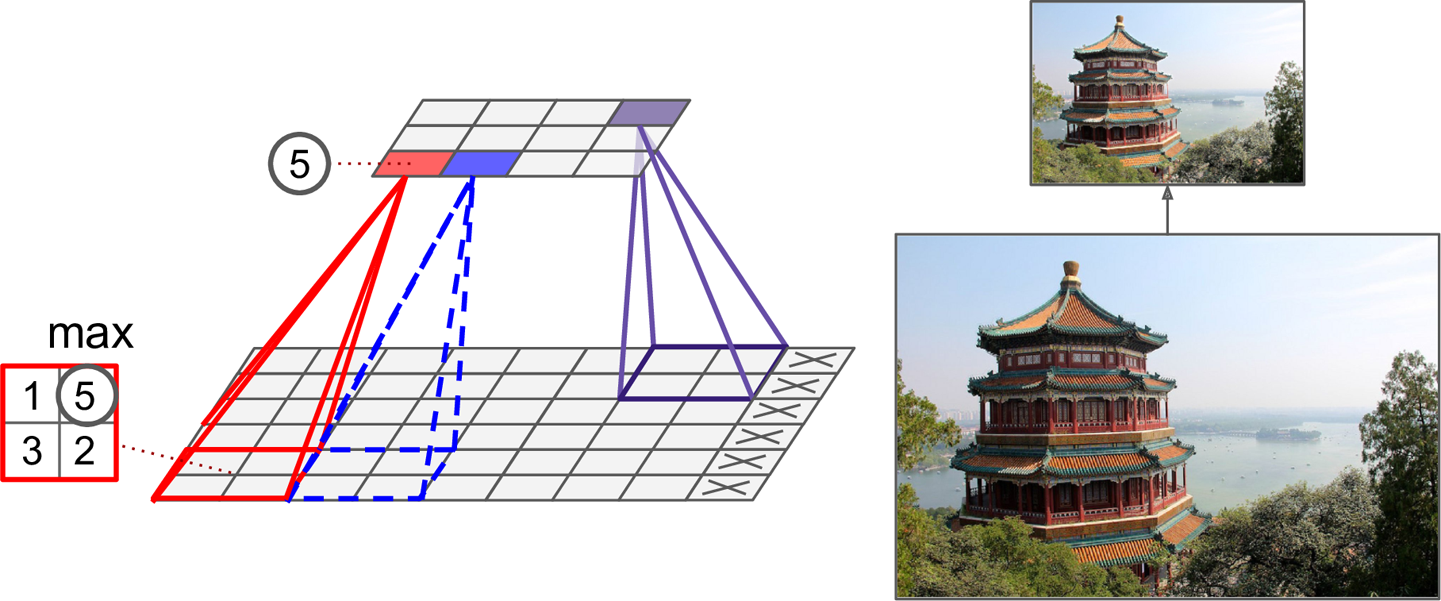
\includegraphics[width=\textwidth]{Images/2-pooling.png}
    \end{center}
    \caption{Ilustración del proceso de agrupación en una red neuronal convolucional usando un kernel de pooling.}
    \label{fig:2-pooling}
\end{figure}

Esta técnica se aplica a cada uno de los mapas de características generados por las capas convolucionales previas, reduciendo efectivamente las dimensiones espaciales mientras se mantiene la profundidad de la entrada \cite{geron2019hands}.

\textbf{e) Arquitecturas}

La arquitectura inicial de las redes neuronales convolucionales (CNN) se remonta a 1995 con la introducción de LeNet. Diseñado por Yann LeCun, este modelo fue pionero en incorporar capas convolucionales para el procesamiento de imágenes \cite{lecun1998gradient}. En los años siguientes, las CNN han experimentado avances significativos, especialmente en el campo de la visión por computadora. Un hito en este desarrollo fue la presentación de AlexNet en 2012 \cite{krizhevsky2012imagenet}, una arquitectura que demostró una mejora sustancial en la precisión de las tareas de clasificación de imágenes en el desafío ImageNet, impulsando así un renovado interés y avance en la investigación en este tipo de redes neuronales \cite{alom2018history}.

Los avances en el campo de las redes neuronales convolucionales han propiciado el desarrollo de diversas arquitecturas especializadas, adaptadas a tareas específicas de procesamiento de imágenes \cite{alom2018history}. En la detección de objetos, modelos como VGG-16, YOLO, Fast R-CNN, Faster R-CNN y ResNet han demostrado ser eficaces. Paralelamente, en la segmentación de objetos, se han empleado con éxito arquitecturas como U-Net, Mask R-CNN, SegNet y DeepLab v3+, abordando desde la segmentación semántica hasta la segmentación por instancia \cite{hoeser2020object, hoeser2020object2}.

En el Cuadro~\ref{tab:ArquitecturasCnn} se presentan las características principales de las arquitecturas de redes neuronales convolucionales más relevantes para la segmentación de objetos.

\begin{table}[H]
    \centering
    \begin{tabular}{|l|l|l|p{6cm}|}
        \hline
        \textbf{Nombre} & \textbf{Año} & \textbf{Creador}            & \textbf{Descripción Detallada}                                                                                                                                                                                                                                                                                                              \\
        \hline
        U-Net           & 2015         & Olaf Ronneberger et al.     & Diseñada para la segmentación biomédica, U-Net destaca por su estructura de codificador-decodificador, que permite trabajar eficazmente con pocos datos de entrenamiento. Su capacidad para combinar contexto y localización precisa la hace ideal para tareas médicas de segmentación de imágenes.                                         \\
        \hline
        SegNet          & 2015         & Vijay Badrinarayanan et al. & SegNet comparte similitudes con U-Net en términos de su estructura de codificador-decodificador, pero se diferencia por tener un decodificador más ligero y por su enfoque en la precisión de los bordes y contornos en la segmentación. Es notable por su uso de pooling índices para mejorar la eficiencia.                               \\
        \hline
        DeepLab         & 2016         & Liang-Chieh Chen et al.     & DeepLab introduce las 'Atrous Convolutions' para captar información contextual en diferentes escalas, lo que mejora notablemente la segmentación. Incluye Atrous Spatial Pyramid Pooling, lo que le permite manejar objetos de distintos tamaños y mejorar la captura de detalles.                                                          \\
        \hline
        Mask R-CNN      & 2017         & Kaiming He et al.           & Mask R-CNN extiende la arquitectura Faster R-CNN agregando una rama para la segmentación de instancias de objetos. Esta arquitectura es capaz de realizar detección de objetos y segmentación de instancias de manera simultánea y precisa, siendo muy influyente en aplicaciones de visión por computadora.                                \\
        \hline
        PSPNet          & 2017         & Hengshuang Zhao et al.      & PSPNet utiliza un 'Pyramid Scene Parsing Network' para integrar características a distintas escalas. Destaca por su habilidad para manejar escenas complejas y su eficacia en la segmentación de detalles finos, gracias a su enfoque en la integración de contexto y detalle.                                                              \\
        \hline
        YOLACT          & 2019         & Daniel Bolya et al.         & YOLACT (You Only Look At Coefficients) es una arquitectura innovadora para la segmentación de instancias en tiempo real. Utiliza un enfoque de coeficientes prototípicos y máscaras de segmentación, permitiendo la segmentación de instancias con alta velocidad y eficacia, abriendo nuevas posibilidades en aplicaciones en tiempo real. \\
        \hline
    \end{tabular}
    \caption{Cronología de las principales arquitecturas de CNN para la segmentación de imágenes.}
    \label{tab:ArquitecturasCnn}
\end{table}



\subsubsection{Redes generativas adversarias (GANs)}

Las redes neuronales de confrontación generativa (en inglés, Generative Adversarial Networks, abreviado como GANs) fueron introducidas por Ian Goodfellow en 2014 \cite{goodfellow2014generative}. Estas redes se basan en la interacción de dos sub modelos distintos: un modelo generativo y un modelo discriminatorio, como se ilustra en la Figura~\ref{fig:GANs}. El modelo discriminatorio se encarga de determinar si una muestra pertenece al conjunto de datos real o ha sido generada artificialmente. Por otro lado, el modelo generativo tiene como objetivo producir muestras que imiten fielmente la distribución de datos original.

\begin{figure}[H]
    \begin{center}
        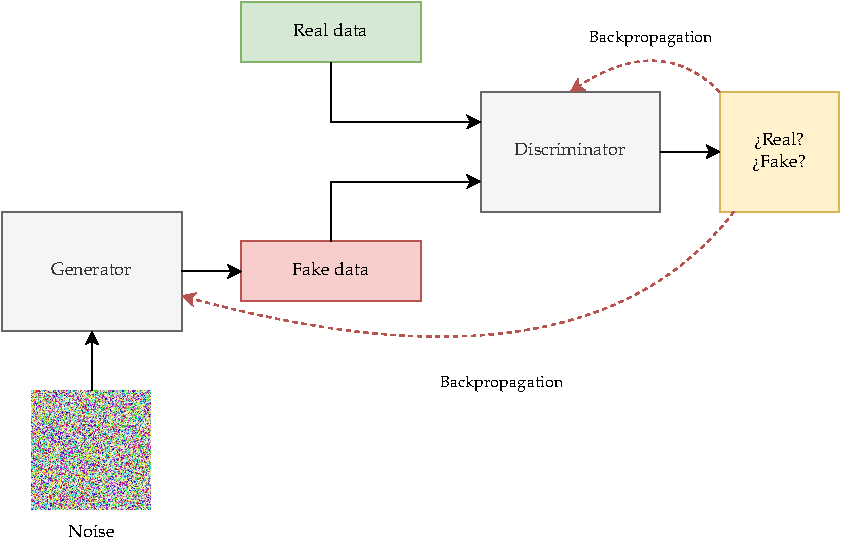
\includegraphics[width=0.7\textwidth]{Images/gan.pdf}
    \end{center}
    \caption{Arquitectura general de una red generativa adversaria.}
    \reference{Elaborado por el autor.}
    \label{fig:GANs}
\end{figure}

El entrenamiento del discriminador implica maximizar la probabilidad de asignar etiquetas correctas tanto a las muestras reales del conjunto de entrenamiento como a las generadas por el generador. De forma paralela, el entrenamiento del generador se enfoca en minimizar la expresión \(\log(1 - D(G(z)))\). En este contexto, la función objetivo óptima para el equilibrio entre el generador y el discriminador se define mediante un juego minimax con una función de valor \(V(G, D)\) dada por:

\begin{equation}
    \underset{G}{min}\:\underset{D}{max}\: \mathbb{E}_{x \sim p_{x}(x)}[\log D(x)] + \mathbb{E}_{z \sim p_{z}(z)} [\log (1-D(G(z)))]
\end{equation}

El análisis teórico de las GANs sugiere que su criterio de entrenamiento puede permitir la recuperación de la distribución de los datos generados. Sin embargo, en la práctica, esta optimización se lleva a cabo mediante un enfoque iterativo y numérico. Según la ecuación previamente mencionada, la optimización de \(D\) en cada ciclo de entrenamiento resultaría computacionalmente inviable y podría causar overfitting en conjuntos de entrenamiento de tamaño limitado \cite{jiang2018deep}.

Para mitigar la inestabilidad durante el entrenamiento de las GANs, se han desarrollado variantes como las GANs de Wasserstein. Estas versiones buscan ofrecer una mayor estabilidad en el proceso de entrenamiento. Se ha observado que el método de Wasserstein converge más rápidamente y produce muestras de mayor calidad en comparación con las GANs tradicionales \cite{arjovsky2017wasserstein}. Actualmente, este tipo de redes neuronales encuentra aplicaciones en diversas áreas, incluyendo transferencia de estilo, generación de imágenes a partir de características condensadas y creación de sonidos, por mencionar algunas \cite{goodfellow2016deep}.
